% Copyright 2004 by Till Tantau <tantau@users.sourceforge.net>.
%
% In principle, this file can be redistributed and/or modified under
% the terms of the GNU Public License, version 2.
%
% However, this file is supposed to be a template to be modified
% for your own needs. For this reason, if you use this file as a
% template and not specifically distribute it as part of a another
% package/program, I grant the extra permission to freely copy and
% modify this file as you see fit and even to delete this copyright
% notice. 

\documentclass{beamer}
% Replace the \documentclass declaration above
% with the following two lines to typeset your 
% lecture notes as a handout:
%\documentclass{article}
%\usepackage{beamerarticle}


% There are many different themes available for Beamer. A comprehensive
% list with examples is given here:
% http://deic.uab.es/~iblanes/beamer_gallery/index_by_theme.html
% You can uncomment the themes below if you would like to use a different
% one:
%\usetheme{AnnArbor}
%\usetheme{Antibes}
%\usetheme{Bergen}
%\usetheme{Berkeley}
%\usetheme{Berlin}
%\usetheme{Boadilla}
%\usetheme{boxes}
%\usetheme{CambridgeUS}
%\usetheme{Copenhagen}
%\usetheme{Darmstadt}
%\usetheme{default}
%\usetheme{Frankfurt}
\usetheme{Goettingen}
%\usetheme{Hannover}
%\usetheme{Ilmenau}
%\usetheme{JuanLesPins}
%\usetheme{Luebeck}
%\usetheme{Madrid}
%\usetheme{Malmoe}
%\usetheme{Marburg}
%\usetheme{Montpellier}
%\usetheme{PaloAlto}
%\usetheme{Pittsburgh}
%\usetheme{Rochester}
%\usetheme{Singapore}
%\usetheme{Szeged}
%\usetheme{Warsaw}
\usepackage[utf8]{inputenc}
\usepackage[catalan]{babel}
\usepackage{ulem}
\usepackage{multicol}
\usepackage{hyperref}

\title{El Far}

% A subtitle is optional and this may be deleted
\subtitle{Un sistema de cerca d'informació per a Amnistia Internacional}

\author{Kenan Rhoton}
% - Give the names in the same order as the appear in the paper.
% - Use the \inst{?} command only if the authors have different
%   affiliation.

\institute[Facultat Informàtica de Barcelona --- UPC] % (optional, but mostly needed)
%{
%  \inst{1}%
%  Department of Computer Science\\
%  University of Somewhere
%  \and
%  \inst{2}%
%  Department of Theoretical Philosophy\\
%  University of Elsewhere}
% - Use the \inst command only if there are several affiliations.
% - Keep it simple, no one is interested in your street address.

\date{}
% - Either use conference name or its abbreviation.
% - Not really informative to the audience, more for people (including
%   yourself) who are reading the slides online

%\subject{Theoretical Computer Science}
% This is only inserted into the PDF information catalog. Can be left
% out. 

% If you have a file called "university-logo-filename.xxx", where xxx
% is a graphic format that can be processed by latex or pdflatex,
% resp., then you can add a logo as follows:

% \pgfdeclareimage[height=0.5cm]{university-logo}{university-logo-filename}
% \logo{\pgfuseimage{university-logo}}

% Delete this, if you do not want the table of contents to pop up at
% the beginning of each subsection:
\AtBeginSection[]
{\begin{frame}<beamer>{}
    \begin{multicols}{2}
        \tableofcontents[currentsection]
    \end{multicols}
  \end{frame}
}

\AtBeginDocument{\addtocontents{toc}{\small}
 \addtocontents{lof}{\small}
}

% Let's get started
\begin{document}

\begin{frame}
    \titlepage{}
\end{frame}

\begin{frame}{}
    \begin{multicols}{2}
        \tableofcontents
    \end{multicols}
  % You might wish to add the option [pausesections]
\end{frame}

% Section and subsections will appear in the presentation overview
% and table of contents.
\section{El projecte}

\subsection{Motivació}

\begin{frame}{Motivació}
    \begin{itemize}
        \item Fer un sistema útil
        \pause{}
        \item Fer un sistema \emph{diferent}
        \pause{}
        \item Fer un projecte a més llarg termini
        \pause{}
        \item Aportar a la societat
    \end{itemize}
\end{frame}

\subsection{Introducció}

% You can reveal the parts of a slide one at a time
% with the \pause command:
\begin{frame}{Introducció}

    
\includegraphics[height=0.2\textheight]{amnesty.jpg}

  \begin{itemize}
    \item Un sistema per cercar informació
    \pause{}% The slide will pause after showing the first item
  
    \item Monitoritzar diferents pàgines web
    \pause{}
  
    % You can also specify when the content should appear
    % by using <n->:
    \item Cerca de paraules clau
    \pause{}
  
    \item Cerca en documents
    \pause{}
  
    % or you can use the \uncover command to reveal general
    % content (not just \items):
    \item Obtenir les notícies d'interés
  \end{itemize}
\end{frame}

\subsection{Descripció del sistema}

\begin{frame}{Descripció del sistema}
    \begin{block}{El Far}
        \begin{itemize}
            \item Cerca d'Avisos automàtica
            \item Gestió de Fonts d'informació
            \item Gestió de Catàlegs de paraules clau
            \item Anàlisi de documents
        \end{itemize}
    \end{block}
\end{frame}

\section{Investigació}

\subsection{Google}

\begin{frame}{Google}
    \begin{block}{Capacitats}
        \begin{itemize}
            \item Cerca d'Avisos \sout{automàtica}
            \item \sout{Gestió de Fonts d'informació}
            \item \sout{Gestió de Catàlegs de paraules clau}
            \item \sout{Anàlisi de documents}
        \end{itemize}
    \end{block}
\end{frame}

\subsection{Versionista}

\begin{frame}{Versionista}
    \begin{block}{Capacitats}
        \begin{itemize}
            \item Cerca d'Avisos automàtica
            \item Gestió de Fonts d'informació
            \item \sout{Gestió de Catàlegs de paraules clau}
            \item \sout{Anàlisi de documents}
        \end{itemize}
    \end{block}
\end{frame}


\subsection{Visualping}

\begin{frame}{Visualping}
    \begin{block}{Capacitats}
        \begin{itemize}
            \item Cerca d'Avisos automàtica
            \item Gestió de Fonts d'informació
            \item \sout{Gestió de Catàlegs de paraules clau}
            \item \sout{Anàlisi de documents}
            \item Falsos positius adicionals!
        \end{itemize}
    \end{block}
\end{frame}


\subsection{Google Docs}

\begin{frame}{Google Docs}
    \begin{block}{Capacitats}
        \begin{itemize}
            \item Cerca d'Avisos automàtica
            \item Gestió de Fonts d'informació
            \item Gestió de Catàlegs de paraules clau
            \item \sout{Anàlisi de documents}
            \item Immens coneixement tècnic requerit per l'usuari
        \end{itemize}
    \end{block}
\end{frame}


\subsection{WebSite-Watcher}

\begin{frame}{WebSite-Watcher}
    \begin{block}{Capacitats}
        \begin{itemize}
            \item Cerca d'Avisos automàtica
            \item Gestió de Fonts d'informació
            \item \sout{Gestió de Catàlegs de paraules clau}
            \item \sout{Anàlisi de documents}
            \item Cuota mensual
        \end{itemize}
    \end{block}
\end{frame}


\subsection{Distill Web Monitor}

\begin{frame}{Distill Web Monitor}
    \begin{block}{Capacitats}
        \begin{itemize}
            \item Cerca d'Avisos automàtica
            \item Gestió de Fonts d'informació
            \item Gestió de Catàlegs de paraules clau
            \item \sout{Anàlisi de documents}
            \item Increiblement senzill!
        \end{itemize}
    \end{block}
\end{frame}


\subsection{El Far}

\begin{frame}{El Far}
    \begin{block}{Conclusió}
        Cap altra eina satisfà completament les característiques cercades.
    \end{block}
\end{frame}

\addtocontents{toc}{\newpage}

\section{Com funciona?}

\subsection{Estructura del sistema}

\begin{frame}{Estructura del sistema}
    \begin{block}{Model de dades}
        \begin{center}
            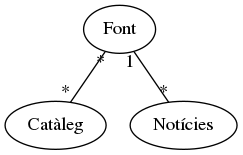
\includegraphics[width=0.6\textwidth]{graph.png}
        \end{center}
    \end{block}
\end{frame}

\subsection{Eines emprades}

\begin{frame}{Eines emprades}{Django}
    \begin{block}{Per què Django?}
        \begin{itemize}
            \item Python
            \pause{}
            \item Molt ben documentat
            \pause{}
            \item Modularitat
            \pause{}
            \item Testabilitat
        \end{itemize}
    \end{block}
\end{frame}

\begin{frame}{Eines emprades}{Heroku}
    \begin{block}{Per què Heroku?}
        \begin{itemize}
            \item Experiència prèvia
            \pause{}
            \item Integració amb Django
            \pause{}
            \item Gestió senzilla a través de CLI
        \end{itemize}
    \end{block}
\end{frame}

\begin{frame}{Eines emprades}{Altres}
    \begin{block}{Mencions especials}
        \begin{itemize}
            \item Vim
            \pause{}
            \item Git
            \pause{}
            \item Redis
            \pause{}
            \item Django File DB Storage
            \pause{}
            \item PyPDF2
        \end{itemize}
    \end{block}
\end{frame}

\subsection{Metodologia}

\begin{frame}{Metodología}
    \begin{block}{Àgil}
        \begin{itemize}
            \item Sprints per funcionalitats
            \item Reunions amb el client
            \item Adaptar el sistema als requisits canviants
        \end{itemize}
    \end{block}
\end{frame}

\begin{frame}{Metodología}
    \begin{block}{TDD}
        \begin{itemize}
            \item Test first
            \item Develop later
            \item Un test per funcionalitat
        \end{itemize}
    \end{block}
    \pause{}
    \begin{alertblock}{Error!}
        No es va respectar des del principi
    \end{alertblock}
\end{frame}

\subsection{Desplegament}

\begin{frame}{Desplegament}
    \begin{block}{Heroku}
        \begin{itemize}
            \item Codi localitzat a \url{mighty-ridge-1447.herokuapp.com}
            \item Desplegat mitjancant Git
            \item Contenidors immutables
        \end{itemize}
    \end{block}
\end{frame}

\section{Problemes i solucions}

\subsection{Heroku i la immutabilitat}

\begin{frame}{Heroku i la immutabilitat}
    \begin{alertblock}{Problema}
        Els contenidors de Heroku són immutables i per tant qualsevol informació guardada al sistema de fitxers es perd.
    \end{alertblock}
    \pause{}
    \begin{exampleblock}{Solució}
        Fer servir la eina Django DB File Storage per guardar els fitxers de referències de les Fonts a la Base de Dades.
    \end{exampleblock}
\end{frame}

\subsection{PDFs}

\begin{frame}{PDFs}
    \begin{alertblock}{Problema}
        Les poques eines que hi han per tractar PDFs en Python no fan el que volem (extreure el text) ni están ben documentades en general.
    \end{alertblock}
    \pause{}
    \begin{exampleblock}{Solució}
        Per sort vam acabar trobant la eina PyPDF2, que tot i no estar massa documentada, permet extreure'n text pla de un arxiu PDF\@.
    \end{exampleblock}
\end{frame}

\subsection{Canvis de paradigmes}

\begin{frame}{Canvis de paradigmes}
    \begin{alertblock}{Problema}
        La solució inicial considerant les Notícies com a seccions concretes de les pàgines web provocava problemes tals com:
        \begin{itemize}
            \item Necessitat de acció concreta (i complexa) de l'usuari per especificar-les
            \item Debilitat a canvis estructurals
        \end{itemize}
    \end{alertblock}
    \pause{}
    \begin{exampleblock}{Solució}
        Es va canviar a la estructura actual d'Avisos, on l'usuari només necessita indicar la Font.
    \end{exampleblock}
\end{frame}

\section{Aprenentatges}

\begin{frame}{Aprenentatges}
    \begin{itemize}
        \item TDD\@!
        \item Familiaritat no és una garantia
    \end{itemize}
\end{frame}

\section{Valoració del client}

\begin{frame}{Valoració del client}
    \begin{itemize}
        \item Objectius bàsics complerts
        \item Gran estalvi de temps amb l'eina
        \item Ús habitual d'ella
        \item Necessitat de manteniment
    \end{itemize}
\end{frame}

\section{Demostració}
\begin{frame}{Demostració}
    \url{http://mighty-ridge-1447.herokuapp.com}

    Codi a \url{https://github.com/kenan-rhoton/far}
\end{frame}

\end{document}
